% Soubory musí být v kódování, které je nastaveno v příkazu \usepackage[...]{inputenc}

\documentclass[%        Základní nastavení
%  draft,    				  % Testovací překlad
  12pt,       				% Velikost základního písma je 12 bodů
  a4paper,    				% Formát papíru je A4
  %oneside,      			% Jednostranný tisk
	twoside,      			% Dvoustranný tisk (kapitoly a další důležité části tedy začínají na lichých stranách)
	unicode,						% Záložky a metainformace ve výsledném  PDF budou v kódování unicode
]{report}				    	% Dokument třídy 'zpráva', vhodná pro sazbu závěrečných prací s kapitolami

\usepackage[utf8]		  %	Kódování zdrojových souborů je UTF-8
	{inputenc}					% Balíček pro nastavení kódování zdrojových souborů

\usepackage[				% Nastavení geometrie stránky
	bindingoffset=10mm,		% Hřbet pro vazbu
	hmargin={25mm,25mm},	% Vnitřní a vnější okraj  (jsou nehezky shodné; jakási úroveň estetiky je dosažena pomocí hřbetu)
	vmargin={25mm,34mm},	% Horní a dolní okraj
	footskip=17mm,			  % Velikost zápatí
	nohead,					      % Bez záhlaví
	marginparsep=2mm,		  % Vzdálenost marginálií
	marginparwidth=18mm,	% Šířka marginálií
]{geometry}

\usepackage{sectsty}
	%přetypuje nadpisy všech úrovní na bezpatkové, kromě \chapter, která je přenastavena zvlášť v thesis.sty
	\allsectionsfont{\sffamily}

\usepackage{graphicx} % Balíček 'graphicx' pro vkládání obrázků
											% Nutné pro vložení logotypů školy a fakulty

\usepackage[          % Balíček 'acronym' pro sazby zkratek a symbolů
	nohyperlinks				% Nebudou tvořeny hypertextové odkazy do seznamu zkratek
]{acronym}						
											% Nutné pro použití prostředí 'acronym' balíčku 'thesis'

\usepackage[
	breaklinks=true,		% Hypertextové odkazy mohou obsahovat zalomení řádku
	hypertexnames=false, % Názvy hypertext. odkazů budou tvořeny nezávisle na názvech TeXu
]{hyperref}						% Balíček 'hyperref' pro sazbu hypertextových odkazů
											% Nutné pro použití příkazu 'pdfsettings' balíčku 'thesis'

\usepackage{pdfpages} % Balíček umožňující vkládat stránky z PDF souborů
                      % Nutné při vkládání titulních listů a zadání přímo
                      % ve formátu PDF z informačního systému

\usepackage{enumitem} % Balíček pro nastavení mezerování v odrážkách
  \setlist{topsep=0pt,partopsep=0pt,noitemsep} % konkrétní nastavení

\usepackage{cmap} 		% Balíček cmap zajišťuje, že PDF vytvořené `pdflatexem' je
											% plně "prohledávatelné" a "kopírovatelné"

%\usepackage{upgreek}	% Balíček pro sazbu stojatých řeckých písmem
											%% např. stojaté pí: \uppi
											%% např. stojaté mí: \upmu (použitelné třeba v mikrometrech)
											%% pozor, grafická nekompatibilita s fonty typu Computer Modern!
                      
%\usepackage{amsmath} %balíček pro sabu náročnější matematiky                 

\usepackage{dirtree}	% sazba adresářové struktury
                      % vhodné pro prezentaci obsahu elektronické přílohy (např. CD)

\usepackage[formats]{listings}	% Balíček pro sazbu zdrojových textů
\lstset{              % nastavení
%	Definice jazyka použitého ve výpisech
%    language=[LaTeX]{TeX},	% LaTeX
%	language={Matlab},		% Matlab
	language={C},           % jazyk C
    basicstyle=\ttfamily,	% definice základního stylu písma
    tabsize=2,			% definice velikosti tabulátoru
    inputencoding=utf8,         % pro soubory uložené v kódování UTF-8
		columns=fixed,  %fixed nebo flexible,
		fontadjust=true %licovani sloupcu
    extendedchars=true,
    literate=%  definice symbolů s diakritikou
    {á}{{\'a}}1
    {č}{{\v{c}}}1
    {ď}{{\v{d}}}1
    {é}{{\'e}}1
    {ě}{{\v{e}}}1
    {í}{{\'i}}1
    {ň}{{\v{n}}}1
    {ó}{{\'o}}1
    {ř}{{\v{r}}}1
    {š}{{\v{s}}}1
    {ť}{{\v{t}}}1
    {ú}{{\'u}}1
    {ů}{{\r{u}}}1
    {ý}{{\'y}}1
    {ž}{{\v{z}}}1
    {Á}{{\'A}}1
    {Č}{{\v{C}}}1
    {Ď}{{\v{D}}}1
    {É}{{\'E}}1
    {Ě}{{\v{E}}}1
    {Í}{{\'I}}1
    {Ň}{{\v{N}}}1
    {Ó}{{\'O}}1
    {Ř}{{\v{R}}}1
    {Š}{{\v{S}}}1
    {Ť}{{\v{T}}}1
    {Ú}{{\'U}}1
    {Ů}{{\r{U}}}1
    {Ý}{{\'Y}}1
    {Ž}{{\v{Z}}}1
}

%%%%%%%%%%%%%%%%%%%%%%%%%%%%%%%%%%%%%%%%%%%%%%%%%%%%%%%%%%%%%%%%%
%%%%%%      !!! VLASTNÍ BALÍČKY A NASTAVENÍ !!!        %%%%%%%%%%
%%%%%%%%%%%%%%%%%%%%%%%%%%%%%%%%%%%%%%%%%%%%%%%%%%%%%%%%%%%%%%%%%
%====== Units =====
\usepackage{siunitx}
\sisetup{inter-unit-product =\ensuremath{\cdot}}
\sisetup{group-digits = integer}
\sisetup{output-decimal-marker = {,}}
\sisetup{exponent-product = \ensuremath{\cdot}}
\sisetup{separate-uncertainty}
\sisetup{tight-spacing = false}
\DeclareSIUnit\permille{\text{\textperthousand}}
%\sisetup{scientific-notation = true}
%\sisetup{round-mode=places,round-precision=4}
%\sisetup{evaluate-expression}

%====== Hyperlinky ====== 
\hypersetup{allbordercolors={1 1 1}}

%====== Obrazky ========
% \usepackage{graphicx} 
% \usepackage[dvipsnames]{xcolor} % E: option clash for package xcolor
% \usepackage{tikz}

% ^^ už tam někde prý jsou použité

\usepackage[siunitx]{circuitikz}
\usepackage{pgf}
\usetikzlibrary{matrix}
\usetikzlibrary{patterns}
\usepackage{tkz-euclide}
\usetikzlibrary{arrows.meta, bending, patterns.meta, ducks}
\usetikzlibrary{shapes, backgrounds, decorations.pathmorphing, calc}

\usepackage{derivative} % nebude potřeba

\usepackage{pgfplots}
\pgfplotsset{width=0.8\linewidth, compat=1.17}
\def\plotcscale{0.8}
\usepackage{pgfplotstable}








%%%%%%%%%%%%%%%%%%%%%%%%%%%%%%%%%%%%%%%%%%%%%%%%%%%%%%%%%%%%%%%%%
%%%%%%      Definice informací o dokumentu             %%%%%%%%%%
%%%%%%%%%%%%%%%%%%%%%%%%%%%%%%%%%%%%%%%%%%%%%%%%%%%%%%%%%%%%%%%%%

% V tomto souboru se nastavují téměř veškeré informace, proměnné mezi studenty:
% jméno, název práce, pohlaví atd.
% Tento soubor je SDÍLENÝ mezi textem práce a prezentací k obhajobě -- netřeba něco nastavovat na dvou místech.

\usepackage[
%%% Z následujících voleb jazyka lze použít pouze jednu
  czech-english,		% originální jazyk je čeština, překlad je anglicky (výchozí)
  %english-czech,	% originální jazyk je angličtina, překlad je česky
  %slovak-english,	% originální jazyk je slovenština, překlad je anglicky
  %english-slovak,	% originální jazyk je angličtina, překlad je slovensky
%
%%% Z následujících voleb typu práce lze použít pouze jednu
  semestral,		  % semestrální práce (výchozí)
  %bachelor,			%	bakalářská práce
  %master,			  % diplomová práce
  %treatise,			% pojednání o disertační práci
  %doctoral,			% disertační práce
%
%%% Z následujících voleb zarovnání objektů lze použít pouze jednu
%  left,				  % rovnice a popisky plovoucích objektů budou zarovnány vlevo
	center,			    % rovnice a popisky plovoucích objektů budou zarovnány na střed (vychozi)
%
]{thesis}   % Balíček pro sazbu studentských prací


%%% Jméno a příjmení autora ve tvaru
%  [tituly před jménem]{Křestní}{Příjmení}[tituly za jménem]
% Pokud osoba nemá titul před/za jménem, smažte celý řetězec '[...]'
\author[]{Jakub}{Charvot}

%%% Identifikační číslo autora (VUT ID)
\butid{240844}

%%% Pohlaví autora/autorky
% (nepoužije se ve variantě english-czech ani english-slovak)
% Číselná hodnota: 1...žena, 0...muž
\gender{0}

%%% Jméno a příjmení vedoucího/školitele včetně titulů
%  [tituly před jménem]{Křestní}{Příjmení}[tituly za jménem]
% Pokud osoba nemá titul před/za jménem, smažte celý řetězec '[...]'
\advisor[Ing.]{Pavel}{Tomíček}[]

%%% Jméno a příjmení oponenta včetně titulů
%  [tituly před jménem]{Křestní}{Příjmení}[tituly za jménem]
% Pokud osoba nemá titul před/za jménem, smažte celý řetězec '[...]'
% Nastavení oponenta se uplatní pouze v prezentaci k obhajobě;
% v případě, že nechcete, aby se na titulním snímku prezentace zobrazoval oponent, pouze příkaz zakomentujte;
% u obhajoby semestrální práce se oponent nezobrazuje (jelikož neexistuje)
% U dizertační práce jsou typicky dva až tři oponenti. Pokud je chcete mít na titulním slajdu, prosím ručně odkomentujte a upravte jejich jména v definici "VUT title page" v souboru thesis.sty.
\opponent[doc.]{Oponent}{Krutý}[Ph.D.]

%%% Název práce
%  Parametr ve složených závorkách {} je název v originálním jazyce,
%  parametr v hranatých závorkách [] je překlad (podle toho jaký je originální jazyk).
%  V případě, že název Vaší práce je dlouhý a nevleze se celý do zápatí prezentace, použijte příkaz
%  \def\insertshorttitle{Zkác.\ náz.\ práce}
%  kde jako parametr vyplníte zkrácený název. Pokud nechcete zkracovat název, budete muset předefinovat,
%  jak se vytváří patička slidu. Viz odkaz: https://bit.ly/3EJTp5A
\title[Autonomous aquarium]{Autonomní akvárium}

%%% Označení oboru studia
%  Parametr ve složených závorkách {} je název oboru v originálním jazyce,
%  parametr v hranatých závorkách [] je překlad
\specialization[Microelectronics and Technology]{Mikroelektronika a technologie}

%%% Označení ústavu
%  Parametr ve složených závorkách {} je název ústavu v originálním jazyce,
%  parametr v hranatých závorkách [] je překlad
%\department[Department of Control and Instrumentation]{Ústav automatizace a měřicí techniky}
%\department[Department of Biomedical Engineering]{Ústav biomedicínského inženýrství}
%\department[Department of Electrical Power Engineering]{Ústav elektroenergetiky}
%\department[Department of Electrical and Electronic Technology]{Ústav elektrotechnologie}
%\department[Department of Physics]{Ústav fyziky}
%\department[Department of Foreign Languages]{Ústav jazyků}
%\department[Department of Mathematics]{Ústav matematiky}
\department[Department of Microelectronics]{Ústav mikroelektroniky}
%\department[Department of Radio Electronics]{Ústav radioelektroniky}
%\department[Department of Theoretical and Experimental Electrical Engineering]{Ústav teoretické a experimentální elektrotechniky}
% \department[Department of Telecommunications]{Ústav telekomunikací}
%\department[Department of Power Electrical and Electronic Engineering]{Ústav výkonové elektrotechniky a elektroniky}

%%% Označení fakulty
%  Parametr ve složených závorkách {} je název fakulty v originálním jazyce,
%  parametr v hranatých závorkách [] je překlad
%\faculty[Faculty of Architecture]{Fakulta architektury}
\faculty[Faculty of Electrical Engineering and~Communication]{Fakulta elektrotechniky a~komunikačních technologií}
%\faculty[Faculty of Chemistry]{Fakulta chemická}
%\faculty[Faculty of Information Technology]{Fakulta informačních technologií}
%\faculty[Faculty of Business and Management]{Fakulta podnikatelská}
%\faculty[Faculty of Civil Engineering]{Fakulta stavební}
%\faculty[Faculty of Mechanical Engineering]{Fakulta strojního inženýrství}
%\faculty[Faculty of Fine Arts]{Fakulta výtvarných umění}
%
%Nastavení logotypu (v hranatych zavorkach zkracene logo, ve slozenych plne):
\facultylogo[logo/FEKT_zkratka_barevne_PANTONE_CZ]{logo/UTKO_color_PANTONE_CZ}

%%% Rok odevzdání práce
\graduateyear{2024}
%%% Akademický rok odevzdání práce
\academicyear{2023/24}

%%% Datum obhajoby (uplatní se pouze v prezentaci k obhajobě)
\date{11.\,11.\,1980} 

%%% Místo obhajoby
% Na titulních stránkách bude automaticky vysázeno VELKÝMI písmeny (pokud tyto stránky sází šablona)
\city{Brno}

%%% Abstrakt
\abstract[%
This thesis delves into the topic of~aquarium automation, aiming to~design custom device for this purpose. A~market survey is~presented with depiction of~existing commercial solutions in~the~field of~automation, also the~essential technology requirements for~efficient aquarium operation are summarized. Regarding the~design of~the~custom device, the~thesis explain the~chosen architecture and takes a~deeper look at~some of~its~parts. The main outcome of~this thesis is the~creation of~an~electrical schematic for the~control unit. The~present work will be followed by a bachelor's thesis, within which the~device will be completed.
]{%
Tato práce se zaměřuje na problematiku automatizace akvárií a jejím cílem je navrhnout vlastní zařízení sloužící tomuto účelu. V práci je proveden trůzkum trhu a popsána již existující komerční řešení věnující se právě automatizaci, také je zde obsaženo shrnutí minimální techniky potřebné pro provoz akvária. Z hlediska návrhu vlastního zařízení je obsažen popis a odůvodnění zvolené architektury, dále se text detailněji věnuje některým dílčím blokům. Výstupem práce je zejména navržené elektrické schéma řídící jednotky. Na tuto práci bude navazovat bakalářská práce, v rámci které bude zařízení dokončeno. 
}

%%% Klíčová slova
\keywrds[%
aquaristics, automation, ESP32, data buses, device design
]{%
akvaristika, automatizace, ESP32, sběrnice, návrh zařízení
}


%%% Poděkování
\acknowledgement{%
Rád bych poděkoval vedoucímu semestrální práce
panu Ing.~Pavlu Tomíčkovi\ za ochotu i trpělivost, kterou se mnou měl po celou dobu tvorby této práce, a za mnoho cenných a podnětných rad k její odborné i formální stránce. Dále děkuji svému kamarádovi Radku Jančičkovi za osvětu v oblasti akvaristiky. 

}%  % do tohoto souboru doplňte údaje o sobě, druhu práce, názvu...

%%%%%%%%%%%%%%%%%%%%%%%%%%%%%%%%%%%%%%%%%%%%%%%%%%%%%%%%%%%%%%%%%%%%%%%%

%%%%%%%%%%%%%%%%%%%%%%%%%%%%%%%%%%%%%%%%%%%%%%%%%%%%%%%%%%%%%%%%%%%%%%%%
%%%%%%     Nastavení polí ve Vlastnostech dokumentu PDF      %%%%%%%%%%%
%%%%%%%%%%%%%%%%%%%%%%%%%%%%%%%%%%%%%%%%%%%%%%%%%%%%%%%%%%%%%%%%%%%%%%%%
%% Při načteném balíčku 'hyperref' lze použít příkaz '\pdfsettings':
\pdfsettings
%  Nastavení polí je možné provést také ručně příkazem:
%\hypersetup{
%  pdftitle={Název studentské práce},    	% Pole 'Document Title'
%  pdfauthor={Autor studenstké práce},   	% Pole 'Author'
%  pdfsubject={Typ práce}, 						  	% Pole 'Subject'
%  pdfkeywords={Klíčová slova}           	% Pole 'Keywords'
%}
%%%%%%%%%%%%%%%%%%%%%%%%%%%%%%%%%%%%%%%%%%%%%%%%%%%%%%%%%%%%%%%%%%%%%%%

\pdfmapfile{=vafle.map}

%%%%%%%%%%%%%%%%%%%%%%%%%%%%%%%%%%%%%%%%%%%%%%%%%%%%%%%%%%%%%%%%%%%%%%%
%%%%%%%%%%%       Začátek dokumentu               %%%%%%%%%%%%%%%%%%%%%
%%%%%%%%%%%%%%%%%%%%%%%%%%%%%%%%%%%%%%%%%%%%%%%%%%%%%%%%%%%%%%%%%%%%%%%
\begin{document}
\pagestyle{empty} %vypnutí číslování stránek

%%% Vložení desek -- od září 2021 na žádost fakulty nepoužíváno
%\includepdf[pages=1]%  buďto generovaných informačním systémem
  %{pdf/student-desky}% název souboru nesmí obsahovat mezery!
%%% NEBO vytvoření desek z balíčku
%%\makecover
%%%
%\oddpage % při dvojstranném tisku přidá prázdnou stránku
%% kazdopádně ale:
%\setcounter{page}{1} %resetovaní čítače stránek -- desky do číslování nezahrnujeme

%% Vložení titulního listu
\includepdf[pages=1]%    buďto generovaného informačním systémem
  {pdf/student-titulka}% název souboru nesmí obsahovat mezery!
%% NEBO vytvoření titulní stránky z balíčku
%\maketitle
%%
\oddpage  % při dvojstranném tisku se přidá prázdná stránka
   
%% Vložení zadání
\includepdf[pages=1]%   buďto generovaného informačním systémem
  {pdf/student-zadani}% název souboru nesmí obsahovat mezery!
%% NEBO lze vytvořit prázdný list příkazem ze šablony
%\patternpage{}%
%	{\sffamily\Huge\centering ZDE VLOŽIT LIST ZADÁNÍ}%
%	{\sffamily\centering Z~důvodu správného číslování stránek}
%%
\oddpage% při dvojstranném tisku se přidá prázdná stránka

%% Vysázení stránky s abstraktem
\makeabstract

% Vysázení stránky s rozšířeným abstraktem
% (pokud píšete práci v češtině či slovenštině, vložení rozšířeného abstraktu zrušte;
%  pro semestrální projekt také není potřeba rozšířený abstrakt uvádět)
% % Vysázení stránky s rozšířeným abstraktem
% (týká se pouze bc. a dp. prací psaných v angličtině, viz Směrnice rektora 72/2017)
\cleardoublepage
\noindent
{\large\sffamily\bfseries\MakeUppercase{Rozšířený abstrakt}}
\\
Výtah ze směrnice rektora 72/2017:\\
\emph{Bakalářská a diplomová práce předložená v angličtině musí obsahovat rozšířený abstrakt v češtině
nebo slovenštině (čl. 15). To se netýká studentů, kteří studují studijní program akreditovaný v
angličtině.}
(čl. 3, par. 7)\\
\emph{Nebude-li vnitřní normou stanoveno jinak, doporučuje se rozšířený abstrakt o rozsahu přibližně 3
normostrany, který bude obsahovat úvod, popis řešení a shrnutí a~zhodnocení výsledků.}
(čl. 15, par. 5)

%%% Vysázení citace práce
\makecitation

%%% Vysázení prohlášení o samostatnosti
\makedeclaration

%%% Vysázení poděkování
\makeacknowledgement

%%% Vysázení obsahu
\tableofcontents

%%% Vysázení seznamu obrázků
% (vynechejte, pokud máte dva nebo méně obrázků)
\listoffigures

%%% Vysázení seznamu tabulek
% (vynechejte, pokud máte dvě nebo méně tabulek)
\listoftables

%%% Vysázení seznamu výpisů kódu
% (vynechejte, pokud máte dva nebo méně výpisů)
\lstlistoflistings

\cleardoublepage\pagestyle{plain}   % zapnutí číslování stránek


%%%%%%%%%%%%%%%%%%%%%%%%%%%%%%%%%%%%%%%%%%%%%%%%%%%%%%%%%%%%%%%%%
%%%%%%%%%            SAMOTNÉ TEXTY PRÁCE             %%%%%%%%%%%%
%%%%%%%%%%%%%%%%%%%%%%%%%%%%%%%%%%%%%%%%%%%%%%%%%%%%%%%%%%%%%%%%%

\chapter*{Úvod}
\phantomsection
\addcontentsline{toc}{chapter}{Úvod}


V dnešní době, kdy jsou na vzestupu fenomény jako chytrá domácnost, \acs{iot} (\acl{iot}) nebo Průmysl 4.0, se na trhu objevuje stále více výrobků, které se snaží automatizovat a zjednodušit různé oblasti našeho života. Tento trend se dnes dotýká nejedné volnočasové aktivity a to včetně akvaristiky. Tu lze samozřejmě provozovat na různé úrovni, ale i majitelé malých domácích akvárií potřebují k provozu svého koníčku relativně velké množství elektroniky. 
Běžnou praxí je, že každé z použitých zařízení je ovládáno buďto zcela ručně nebo, pokud disponuje možností vzdáleného přístupu a automatizace, má svou samostanou aplikaci a uživatel tak provoz akvária musí ovládat z několika různých míst, což může být značně nepohodlné a nepřehledné.

Na trhu samozřejmě existují také velmi sofistikované a komplexní systémy, ty ovšem svou cenou vysoce přesahují rozpočet běžného "domácího" akvaristy. Tato práce se věnuje návrhu a tvorbě zařízení, které má za cíl nabídnout pohodlnou kontrolu a ovládání všech potřebných součástí domácího akvária, a to při zachování jednoduchosti a nízké pořizovací ceny.

% \input{text/images/CMOS_images.tex}

\chapter*{Cíle práce}
\phantomsection
\addcontentsline{toc}{chapter}{Cíle práce}

Má tato kapitola existovat a nebo mám cíle podrobněji rozebrat v~úvodu? 

\chapter{Základní teorie akvaristiky}
    Tato kapitola je teoretickou částí práce, která předchází návrhu samotného zařízení. Na základě dostupných zdrojů jsou zde rozebrány technické požadavky na provoz akvária a proveden průzkum trhu v oblasti akvaristiky a její automatizace.  

\section{Historie}
    Pro lepší orientaci čtenáře ve trendech vývoje akvaristiky se práce nejprve zaměřuje na krátké shrnutí její historie. Kapitola slouží taképro pochopení motivace akvaristů k~rozvoji používané techniky.
\subsection{Počátky}
Akvaristika v~různých podobách provází lidstvo téměř od prvopočátku. Nejprve se jednalo spíše o~chov ryb užitkových, tedy rybářství, ovšem už ve starověké Mezopotámii docházelo také k~chovu ryb okrasných. Počátky akvaristiky byly prováděny spíše metodou pokusů a omylů, protože lidem nebyla známa velká část přírodních zákonitostí -- životní potřeby chovaných ryb, způsob jejich rozmnožování a v~neposlední řadě také procesy, odehrávající se v~přírodním ekosystému, zajišťující jeho rovnováhu. Základem udržení chovaných ryb naživu byla zejména častá výměna vody, ani tak ale dlouho nebylo možné udržet ryby při životě dlouhodobě. 

V~období středověku se poprvé objevuje také dovoz exotických okrasných rybek z~cizích zemí, pro naprostý nedostatek znalostí ale často brzy hynou, např. jen proto, že chovatele nenapadne je nakrmit~\cite{vitek_akvaristika}.

\subsection{Věda a technika}
Na konci 18. století dochází k~rozvoji vědy a několika objevům, které historii akvaristiky zásadně ovlivnily. Poprvé byl izolován kyslík, byl objasněn princip dýchání živočichů a následně také fotosyntéza. Akvaristika, v~tehdejší době umělý chov ryb za účelem pozorování a výzkumu, byla provozována zejména na vědecké půdě a byl zde zájem o~zdokonalení používaných technik a postupů. V~roce 1837 S. H. Ward prakticky prokázal, že osvětlené akvárium obsahující jak rybky, tak i rostliny, vydrží velmi dlouho bez nutnosti výměny vody~\cite{vitek_akvaristika}. Pricip výměny plynů byl významným milníkem ve snaze dosáhnout v~akváriu rovnováhy podobné přírodnímu prostředí. 

Při stále nových poznatcích o~životních potřebách ryb a o~akvarijní rovnováze bylo nutné přijít s~různými technickými řešeními. Akvária 19. a 20. století už byla vytápěná a uměle okysličovaná. Původní mechanická řešení a lihové kahany byly postupně nahrazovány elektrickými přístroji. V~pozdějších letech pak přibylo i umělé osvětlení a systémy filtrace vody. 
\section{Rozdělení akvárií}
TODO
\section{Technické vybavení akvária}
    V~této kapitole je uveden výčet základní akvaristické techniky nutné k~provozu domácího akvária, rozčleněné podle svého účelu. Ve druhé části se text věnuje přehledu různých dostupných komplexních systémů zaměřujících se na automatizaci provozu akvária. Cílem kapitoly je seznámit čtenáře blíže s~problematikou založení a provozu akvária a různými možnostmi technického zajištění jak domácích, tak i profesionálních akvárií.
    \subsection{Filtrace vody}
        Úkolem filtru je průběžně odstraňovat z~vody nečistoty, a to jak mechanické, tak zejména v~podobě škodlivých látek vznikajících v~akváriu. Filtrační materiál je volen tak, aby tvořil vhodné prostředí pro život filtračních bakterií, které se těmito škodlivými látkami živí \cite{yt-filtrace}. Rozlišujeme tři základní typy akvarijních filtrů -- vnější, vnitřní a závěsné. Na obr.~\ref{fig:filtry-srovnani} se nachází ukázka vybraných zástupců jednotlivých typů.
        
        \textbf{Vnějším filtrem} se rozumí zařízení umístěné obvykle ve skříňce pod akváriem, mívá připojeny dvě hadice -- na vstup a výstup vody. Toto řešení je považováno za nejlepší, protože filtr není omezen rozměry a může tak dosahovat daleko vyššího výkonu a účinnější filtrace díky většímu množství filtračních materiálů. 

        \textbf{Vnitřní filtr} (někdy také ponorný) je levným, ale nepříliš účinným řešením pro malá akvária. Nachází se z~velké části v~akváriu a za pomocí motorku tlačí vodu přes obvykle molitanovou náplň.

        \textbf{Závěsný filtr}  je kompromisním řešením.  Cenou i účinností filtrace se pohybuje mezi oběma zmíněnými typy. Nezabírá prostor uvnitř akvária a může tak využít větší objem filtrační hmoty než filtr vnitřní. Instalace je provedena zavěšením na stěnu akvária, je tedy velmi jednoduchá. 

        \begin{figure}[h!]
            \centering
            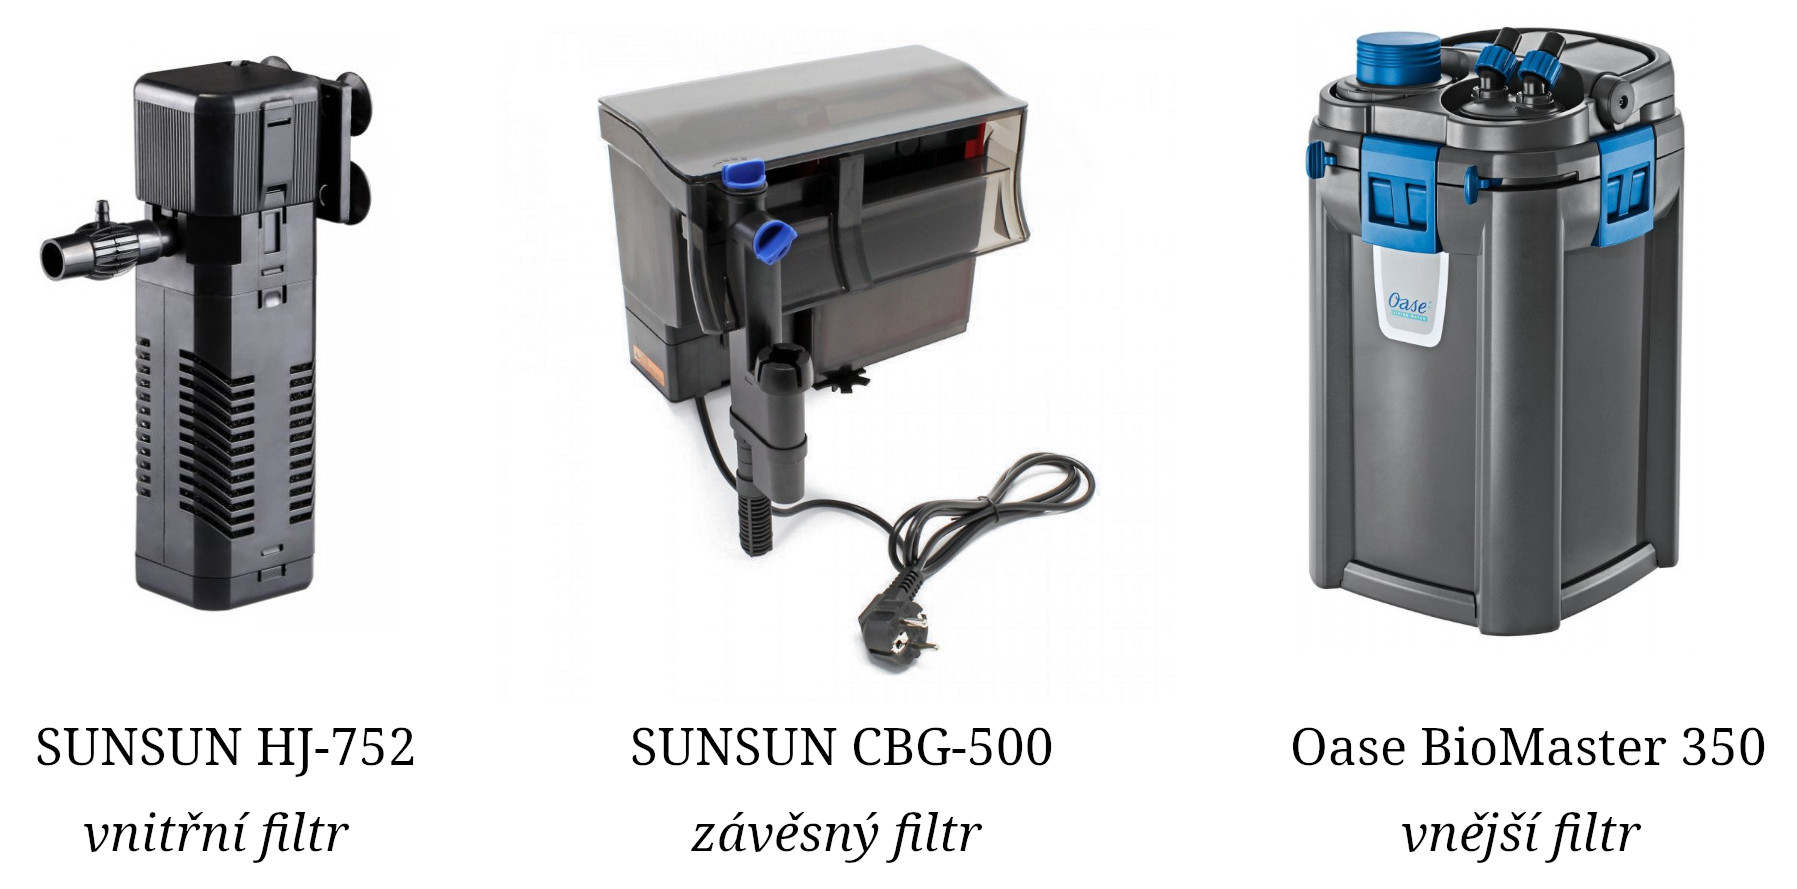
\includegraphics[width=\textwidth]{obrazky/filtry/filtry.jpg}
            \caption{Příklad různých typů filtrů. Převzato z~\cite{eshop-rostlinna-akvaria}.}
            \label{fig:filtry-srovnani}
        \end{figure}

    \subsection{Osvětlení}
        Funkce osvětlení akvária je dvojí. Jednak jde o~estetický dojem z~pohledu pozorovatele, kdy vhodné nasvícení přidává akváriu na atraktivitě. Druhak se osvětlení snaží nasimulovat osazenstvu akvária přirozené životní podmínky, aby celý ekosystém mohl fungovat.

        Hlavními parametry při výběru svítidla jsou jeho \textbf{intenzita}, \textbf{spektální charakteristika} a \textbf{spotřeba}. 
        
        Příliš intenzivní světlo zvyšuje riziko nežádoucí tvorby řas a pro ryby může být stresovým faktorem, nízká intenzita zase může způsobit špatný růst rostlin~\cite{KejzlarRadim2022Ařpa}. Na internetu existuje mnoho návodů a rad na stanovení správné intenzity, ale protože zde hraje roli spousta dalších parametrů jako např. výška hladiny nebo konkrétní typ rostlin, je vhodné tyto hodnoty brát pouze jako orientační a intenzitu osvětlení upravit během provozu podle potřeby. Výpočet se také liší pro jednotlivé typy svítidel. 

        Spektrum světla hraje roli hned z~několika důvodů. Rostliny pro tvorbu chlorofylu a následnou fotosyntézu potřebují světlo zejména vlnových délek \qty{440}{nm} (modrá barva) a \qty{660}{nm} (červená barva)~\cite{eshop-ledsolution-svetlo}, pokud by zvolené osvětlení tyto vlnové délky neobsahovalo, nemohou rostliny správně fungovat. Akvárium osvětlené pouze těmito dvěma barvami by ale nevypadalo vizuálně dobře, proto se využívá také širokospektrální bílé světlo, které svým spektrem odpovídá co nejlépe dennímu světlu. 
        Specializovaná svítidla pak nabízejí možnost napodobit světelné spektrum různých vodních prostředí a přizpůsobit se tak i rostlinám a živočichům žijícím ve velkých hloubkách. 

 
        \begin{figure}[h!]
            \centering
            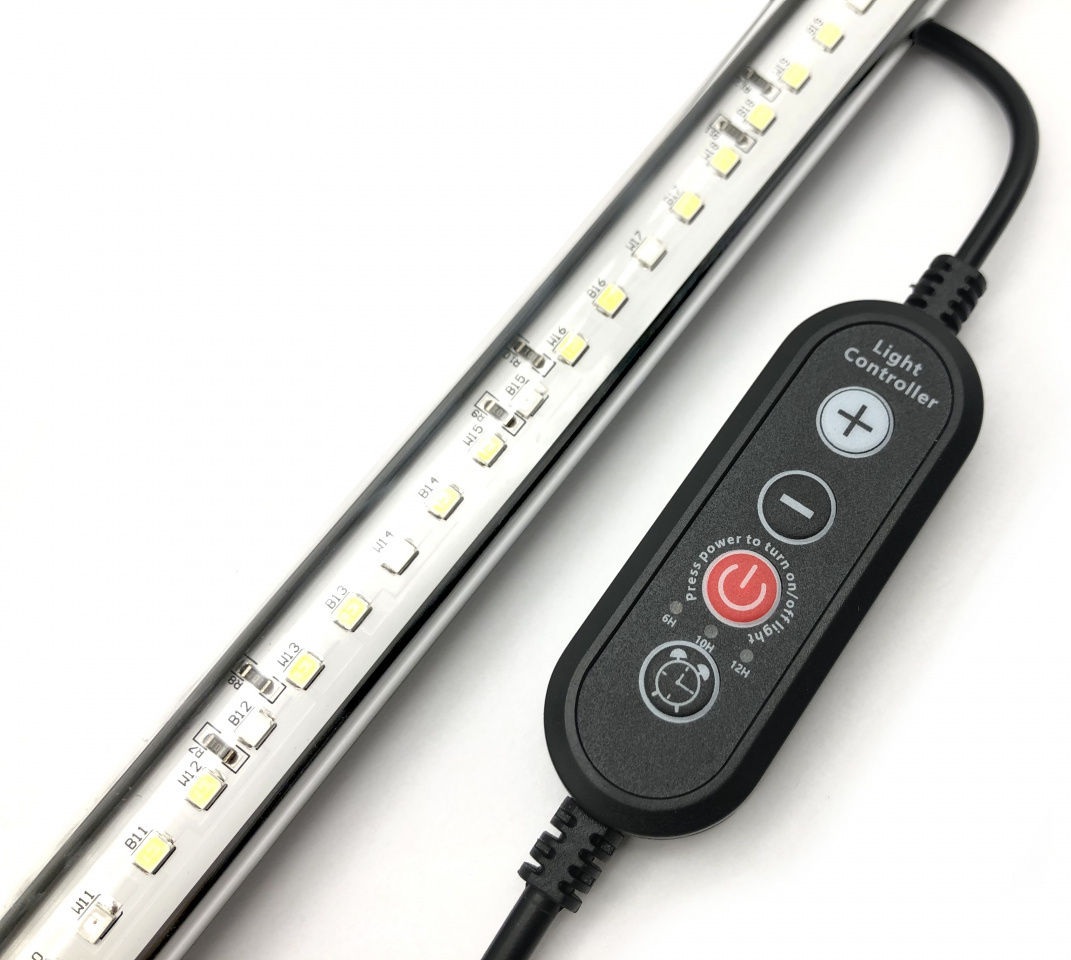
\includegraphics[width=0.5\textwidth]{obrazky/osvetleni/stmivac.jpg}
            \caption{Trubice s~\acs{led} páskem a manuální stmívač a časovač. Převzato z~\cite{eshop-rostlinna-akvaria}.}
            \label{fig:obrazky-osvetleni-stmivac-jpg}
        \end{figure}

        Na trhu jsou v~současné době tři typy akvaristických světel: \textbf{zářivky}, \textbf{výbojky}  a \textbf{\acs{led} svítidla}~\cite{eshop-rostlinna-akvaria-svetlo}. Zářivky jsou považovány za dnes již nepříliš moderní řešení a bývají nahrazovány \acs{led} svítidly, ty se vyznačují lepší účinností (tedy nižší spotřebou energie při stejné intenzitě světla), delší životností a širší paletou barev. U~zářivek také nebylo možné plynule regulovat intenzitu, jako je tomu u~\acs{led}, a dosáhnout tak např. postupného rozsvícení nebo zhasnutí světla simulujícího východ a západ slunce. Skoková změna při zapnutí nebo vypnutí světla je pro ryby také zbytečným stresovým faktorem~\cite{MusilLibor2018Isps}. Co se týče výbojek, ty nacházejí uplatňení zejména pro hluboké nádrže, protože jejich světlo je bodové a intenzita dostačující k~prosvícení velkého objemu vody, spotřeba energie je ale v~porovnání s~\acs{led} vysoká, takže pokud to není nezbytně nutné, je lepší se jim vyhnout.   

        Typické domácí akvárium je osvětleno jedním nebo několika samostatně stmivatelnými \acs{led} svítidly, a to buďto v~podobě \acs{led} pásků nalepených na hliníkovém profilu anebo hotového svítidla, ve kterém jsou čipy s~\acs{led} zabudovány napevno. Stmívání je nastavováno buď ručně anebo za pomoci mobilní aplikace dodané výrobcem stmívače. Příklad běžně dostupného výrobku lze vidět na obr.~\ref{fig:obrazky-osvetleni-stmivac-jpg}.

    \subsection{Ohřev}
        Většina okrasných sladkovodních ryb běžně chovaných akvaristy pochází z~tropických krajů a vyžaduje teplotu vody v~rozmezí 22 -- \qty{26}{\degreeCelsius}~\cite{slavotinek2014}, to je o~něco málo vyšší teplota než bývá v~domácnosti typická a proto je nutné zajistit akváriu možnost dodatečného ohřevu. Nejčastějsím řešením je ponorné topné těleso na odporové bázi s~vlastní termostatovou regulací, viz obr.~\ref{fig:obrazky-topeni-topitko-jpg}.

        \begin{figure}[h!]
            \centering
            \begin{tikzpicture}
                % Include the image
                \node[anchor=south west,inner sep=0] (image) at (0,0) {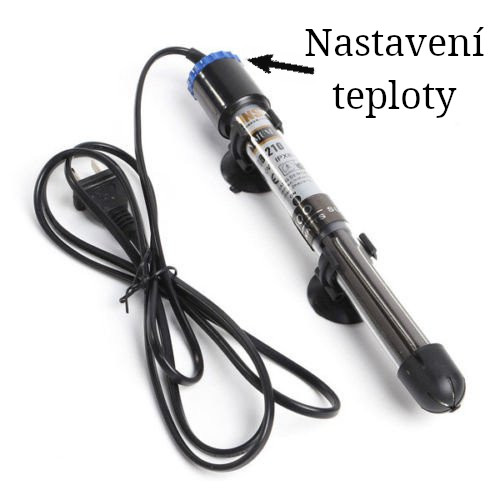
\includegraphics[width=0.5\textwidth]{obrazky/topeni/topitko.jpg}};

                \node (termostat) at (3.8,6.5) {};
                \node[align=center] (napis) at (6,6.5) {Nastavení\\teploty};
                \draw[->] (napis) -- (termostat);
                
            \end{tikzpicture}

            \caption{SUNSUN topítko 100W s~termostatem. Převzato z~\cite{eshop-rostlinna-akvaria}.}
            \label{fig:obrazky-topeni-topitko-jpg}
        \end{figure}
        
        Z~principu fungování termostatu vyplývá, že výsledná teplota vody není v~čase konstantní, ale osciluje okolo nastavené hodnoty. Rozsah kolísání teploty je pak závislý na hysterezi termostatu, obecně lze říci, že to může být i několik stupňů. Pro většinu aplikací to není velký problém, ale některé druhy ryb mohou být na změny teploty náchylnější, v~takovém případě je potřeba buďto vybrat topítko takové, kde výrobce rozsah teplot uvádí, anebo zvolit jiný způsob regulace. 

    \subsection{Monitorování}
    \label{sec:monitorovani}
        Jak již vyplynulo z~úvodních kapitol, v~akváriu probíhá celá řada procesů ovlivňujících jeho stav. Klíčem k~vytvoření prosperujícího akvária je dosažení rovnováhy a stability mezi nimi za pomoci vhodně nastavené akvarijní techniky. Nejen u~začínajících akvaristů se mohou vyskytnout problémy s~růstem rostlin, zdravím ryb nebo třeba výskytem řasy. Odhalit příčiny těchto problémů může být mnohdy obtížné, ovzláště pokud není k~dispozici dostatečné množství informací o~tom, co se v~akváriu děje. 
        
        Existuje několik veličin, které úzce souvisí s~procesy v~akváriu a které je možné také poměrně jednoduše sledovat. Na trhu je celá řada produktů sloužících k~tomuto účelu. Většinou je na výběr možnost analogového nebo čistě mechanického přístroje případně samostatného digitálního čidla, existují ale také komplexní řešení, těm se dále věnuje kapitola  \ref{lab:kapitola-komplexni-reseni}. 

        \subsubsection{Teplota}
            Umístěním teploměru (ať už v~analogové nebo digitální podobě) do akvária je možné zkontrolovat správné nastavení topného tělesa a následně provést jeho úpravu. Také lze včas získat informaci o~jeho případné poruše a nebo třeba jen nedostatečném výkonu. 
        \subsubsection{\acs{ph} a CO\(\mathbf{_{2}}\)}
            Hodnota \acs{ph} popisuje kyselost resp. zásaditost měřeného vodného roztoku. Běžně se používá logaritmická stupnice s~hodnotami 0 až 14, přičemž zcela neutrální voda má \acs{ph} rovno 7, menší hodnoty mají roztoky kyselé a větší než 7 pak roztoky zásadité.  Obecně lze říci, že pro ryby je vyhovující \acs{ph} v~rozsahu 6 až 8~\cite{slavotinek2014}. 

            Důležitým parametrem vody z~pohledu rostlin a ryb je koncentrace \acs{co2}. Přirozeně platí, že rostliny \acs{co2} spotřebovávají při fotosyntéze a jistá koncentrace je tedy nutná pro jejich prosperitu, naopak příliš vysoká koncentrace může být nebezpečná pro ryby, kterým (obdobně jako např. lidem) komplikuje dýchání. Obsah \acs{co2} ve vodě je obtížné přímo měřit, jeho měnící se koncentrace má ale vliv právě na hodnoty \acs{ph}, s~rostoucí koncentrací \acs{co2} se \acs{ph} vody snižuje a obráceně~\cite{DvorakJan2014RPpa,KejzlarRadim2022Ařpa}. 

            K~měření \acs{ph} vody se používají různé chemické testy (kapkové testy, testovací papírky), které je možné zakoupit v~chovatelských potřebách. Z~pohledu automatizace je mnohem zajímavějším řešením \acs{ph} sonda, která umožňuje nepřetržité měření této veličiny a případnou okamžitou regulaci dávkování \acs{co2}.

             
    \subsection{Dostupná komplexní řešení}
    \label{lab:kapitola-komplexni-reseni}
        Tato sekce se věnuje porovnání několika nejznámějších systémů v~oblasti automatizace akvárií. Je důležité připomenout, že ve všech oblastech elektrotechniky dochází k~rychlému rozvoji a každý rok se na trhu objevují nové produkty se stále lepšími parametry a nižší cenou. Informace uvedené v~této kapitole, a to zejména cenové údaje, se mohou velmi rychle stát neaktuálními a jsou tedy relevantní pouze v~době vzniku této práce.

        Při tvorbě této kapitoly byly jako zdroj informací použity jednak oficiální materiály výrobců, ty ovšem samozřejmě obsahují vždy pouze pozitivní informace, dále pak různé uživatelské recenze na platformě YouTube popř. diskuzních fórech, nejedná se o~zcela seriózní zdroje a proto je nutné také informace z~této kapitoly brát s~rezervou. 

        % TODO: Tento obr. až v GHL kapitole - nebudu, NEBUDU TO DĚLAT !!
        \begin{figure}[h!]
            \centering
            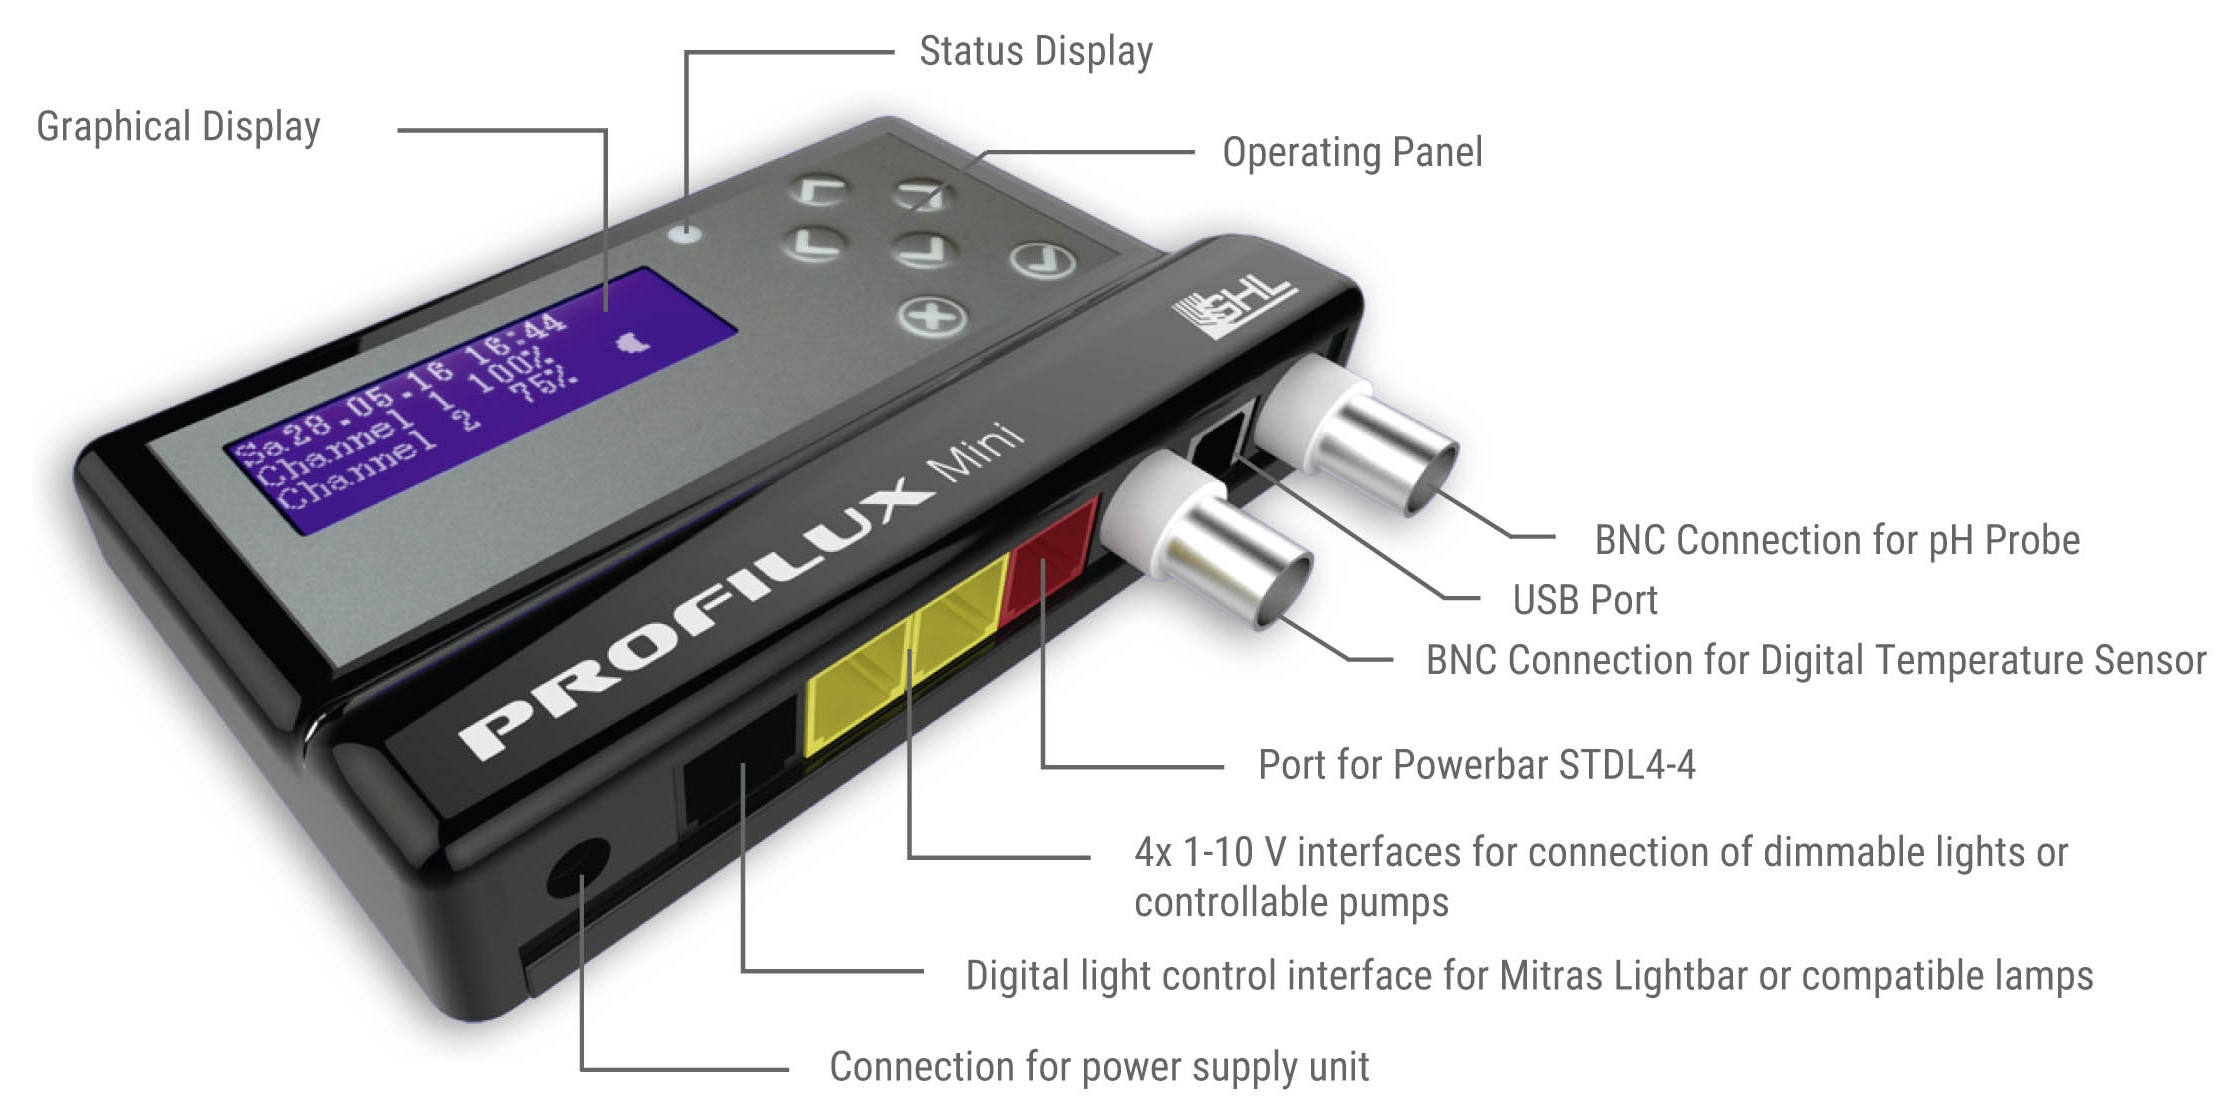
\includegraphics[width=0.9\textwidth]{obrazky/trh/GHL-ProfiLux-Mini.jpg}
            \caption{GHL ProfiLux Mini, nejmenší dostupný kontrolér této firmy. Převzato z~\cite{ghl-profilux}.}
            \label{fig:obrazky-trh-GHL-ProfiLux-Mini-jpg}
        \end{figure}
        \subsubsection{GHL -- ProfiLux}
            Německá firma GHL se v~oblasti akvaristiky pohybuje již přes 20 let a patří nepochybně ke špičce na trhu z~hlediska komplexity a spolehlivosti. Základem jejich systému ProfiLux je kontrolér (např. nejmenší varianta viz obr.~\ref{fig:obrazky-trh-GHL-ProfiLux-Mini-jpg}), který je možné konfigurovat z~PC za pomocí kabelu anebo vzdáleně s~použitím aplikace nebo webového rozhraní. Ke kontroléru lze připojit celou řadu periferíí z~portfolia firmy, jedná se o~různé typy senzorů, dávkovače (pro úpravu parametrů vody), pumpy nebo řiditelný prodlužovací přívod pro síťové zásuvky (laicky řečeno \uv{chytrá prodlužovačka}). Společnost si zakládá na opravdu vysoké kvalitě a přesnosti svých výrobků, což se ale odráží také na jejich ceně. 

            Na výběr je z~několika variant systému, přičemž ty nejdražší dokážou obsloužit i opravdu rozsáhlé a náročné akvaristické instalace. Cena nejlevnějšího základního setu je přibližně od \qty{10000}{Kč}~\cite{ghl-profilux,eshop-ghl-profilux-sets}.

            
        \subsubsection{Neptune Systems -- Apex}
            Systém Apex je nepochybně další ze světových leaderů v~této oblasti. Opět je k~dispozici několik variant systému podle požadavků a finančních možností uživatele a systém je také velmi modulární. Stejně jako firma GHL, i Neptune Systems je na trhu více než 20 let a jedná se tedy o~léty ověřenou značku. Architektura systému je podobná a kromě samotného kontroléru je opět v~nabídce celá řada kompatibilních periferií. Dle uživatelských recenzí je konfigurace systému oproti GHL výrazně jednodušší a není nutná znalost programování, navíc systém už od výroby obsahuje přednastavené nejčastější scénáře použití.

            \begin{figure}[h!]
                \centering
                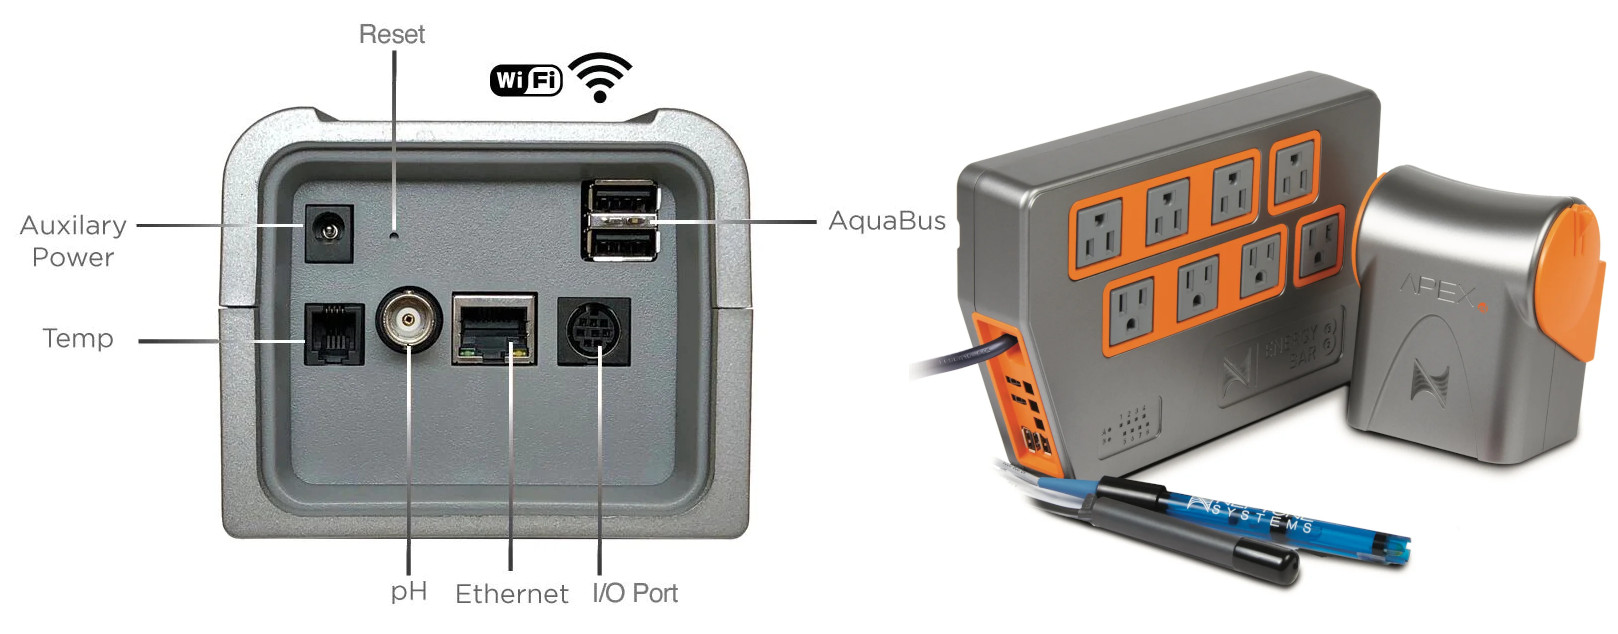
\includegraphics[width=0.8\textwidth]{obrazky/trh/apex-el.jpg}
                \caption{Neptune Systems Apex EL, základní set. Převzato z~\cite{eshop-neptune-systems-apex}.}
                \label{fig:obrazky-trh-apex-el}
            \end{figure}
            
            Cena opět závisí na množství zakoupených modulů, základní set s~podobnou výbavou jako u~GHL je k~dispozici přibližně od \qty{12000}{Kč}~\cite{neptune-systems-why-apex,eshop-neptune-systems-apex}.

        \subsubsection{CoralVue -- HYDROS}
            Firma CoralVue se svým systémem HYDROS je na trhu oproti svým konkurentům relativně krátce, přibližně 3 roky, svým originálním přístupem a cenově dostupným řešením si ale své zákazníky našla rychle. Systém je svou architekturou ještě více modulární než jeho konkurenti, umožňuje v~rámci jedné aplikace spojit i více kontrolérů, které mezi sebou komunikují. Dokonce v~případě poruchy hlavního kontroléru dokáže jeho roli převzít jiný připojený kontrolér a systém tak zůstane dále v~provozu. 
            
            Kromě bezdrátově řízeného modulu se čtyřmi síťovými zásuvkami nově firma nabízí také modul Control XP8, který krom zásuvek obsahuje i vlastní kontrolér, může tak fungovat zcela samostatně, stále však umožňuje také drátové spojení s~dalšími kontroléry nebo bezdrátové připojení k~dalším zásuvkám. Toto může sloužit jako jednoduché univerzální řešení pro menší akvária s~možností budoucího rozšíření. 

            \begin{figure}[h!]
                \centering
                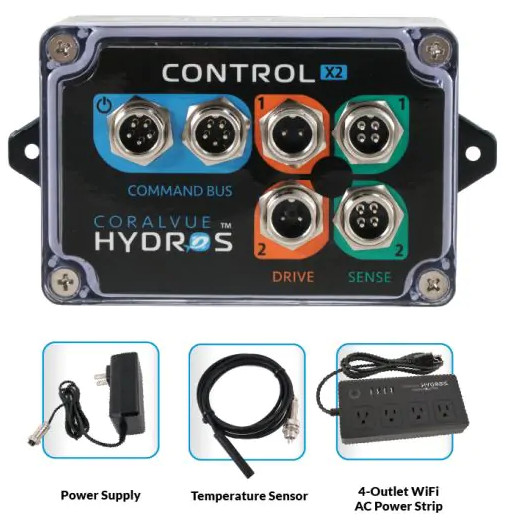
\includegraphics[width=\textwidth]{obrazky/trh/hydros-x2-starter-pack.jpg}
                \caption{CoralVue HYDROS Control X2 Starter pack. Převzato z~\cite{eshop-coralvue-hydros}.}
                \label{fig:obrazky-trh-hydros-x2-starter-pack-jpg}
            \end{figure}
            
            Základní minimální sada je dostupná již od přibližně \qty{4500}{Kč}, aby byla ale výbava stejná jako u~výše zmíněných konkurentů je potřeba dokoupit ještě \acs{ph} sondu za přibližně \qty{800}{Kč}~\cite{coralvuehydros,eshop-coralvue-hydros}.
            
        \subsubsection{Seneye}
            Společnost Seneye nenabízí komplexní řešení pro automatizaci, ale i přesto jsou její produkty zajímavé a pro mnoho akvaristů mohou být skutečně užitečné. Místo pokročilého ovládání akvarijní techniky se výrobky zaměřují pouze na monitorování parametrů vody (popř. dalších veličin), důraz je kladen na maximální jednoduchost použití. 
            
            \begin{figure}[h!]
                \centering
                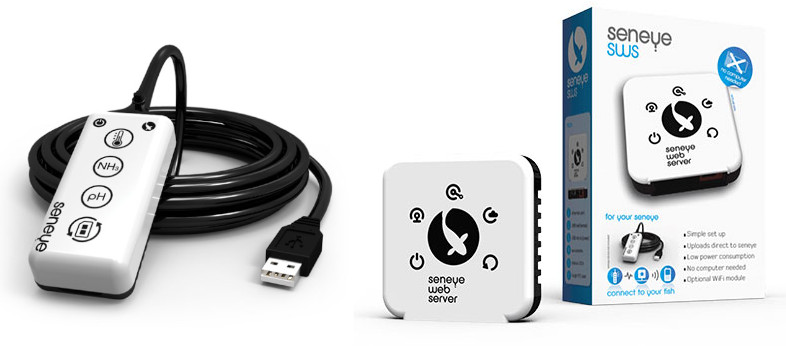
\includegraphics[width=0.6\textwidth]{obrazky/trh/seneye-home.jpg}
                \caption{Seneye Home a Seneye Web Server. Převzato z~\cite{seneye-home}.}
                \label{fig:obrazky-trh-seneye-home-jpg}
            \end{figure}

            Vnitřním sladkovodním akváriím je věnována řada Seneye Home a veškeré monitorování je zajištěno jedním malým zařízením, které uživatel přímo ponoří do vody a pomocí kabelu připojí k~počítači ze kterého se zařízení napájí a zároveň do něj odesílá data. Alternativně lze přikoupit také krabičku, která slouží jako webserver, do ní se zařízení připojí namísto počítače a data jsou rovnou zálohována do cloudu, odkud jsou uživateli dostupná v~mobilní aplikaci. Ukázkové foto je na obr.~\ref{fig:obrazky-trh-seneye-home-jpg}.

            Zařízení monitoruje teplotu, \acs{ph}, úroveň škodlivého amoniaku, osvětlení a hladinu vody. Umožňuje také odesílat oznámení při překročení nastavené meze některého z~parametrů.

            Cena samotného monitorovacího zařízení je přibližně \qty{3000}{Kč} a podobná je také cena zmíněného webserveru. Pro automatické monitorování se zálohou na cloud je tedy potřeba počítat s~investicí okolo \qty{6000}{Kč}~\cite{seneye-home}.
            


        









\chapter{Systémový návrh}

Tato část práce popisuje proces tvorby návrhu výsledného zařízení, věnuje se konkretizaci požadavků na zařízení a následnému hledání vhodných technických řešení pro tyto požadavky včetně výběru odpovídajících komponent.

\section{Požadavky}
\label{sec:pozadavky}
    Cílem je vytvořit zařízení, které umožní co nejvíce automatizovat provoz akvária. Hlavním aspektem by měla být jednoduchost použití pro koncového uživatele, vše by mělo být nanejvýš intuitivní a přehledné. Zařízení musí mít možnost připojení k~internetu prostřednictvím sítě Wi-Fi, uživatel tak bude moci zařízení konfigurovat a sledovat z~libovolného místa za pomoci webové stránky popř. mobilní aplikace.

    Požadavky jednotlivých akvaristů se mohou lišit a zároveň se v~čase měnit. Vytvoření dokonalého a všestaranného zařízení, které vyhoví všem účelům použití není v~časových ani finančních možnostech bakalářské práce, proto byl stanoven požadavek, aby bylo zařízení co nejvíce modulární a rozšiřitelné. Musí být zvolena taková architektura, aby bylo možné v~budoucnu přidat další funkce a periferie bez nutnosti modifikovat stávající hardware.

    Výstupem bakalářské práce by mělo být zařízení schopné monitorovat některé akvaristické veličiny a na základě jejich hodnoty informovat uživatele a ovládat akvárium. Zařízení bude přímo řídit \acs{led} páskové osvětlení na \qty{12}{V} a spínat popř. vypínat již existující akvaristické přístroje pracující se síťovým napětím \qty{230}{V}.  

    Jelikož modulární architektura bude nepochybně vyžadovat použití více než jednoho mikrokontroléru a tedy také více různých firmwarů, je potřeba zajistit jejich vzájemnou kompatibilitu a stabilitu celého systému. Veškerý firmware tak musí být verzovaný a po připojení nové periferie musí řídicí jednotka rozpoznat, o~jakou periferii se jedná. V~případě připojení nekompatibilní periferie (např. z~důvodu zastaralého firmwaru řídicí jednotky) musí být uživatel upozorněn a nesmí být nijak narušena funkce zbytku systému. Aby bylo možné těmto situacím předejít, musí mít řídicí jednotka možnost vzdálené aktualizace firmwaru.
\section{Koncepční schéma}
\section{Návrh komunikačního rozhraní}
\section{Výběr komponent}

\subsection{Řídící jednotka}

\subsection{Periferie}












\chapter{Tvorba elektrického schématu}

\section{Řídící jednotka}
\section{Modul pro LED osvětlení}
\section{Senzory}
    \subsection{Teploměr}
    \subsection{Senzor výšky hladiny}
\section{Modul pro ovládání \qty{230}{V} periferií}














\chapter*{Závěr}
\phantomsection
\addcontentsline{toc}{chapter}{Závěr}

V~rámci bakalářské práce bylo navrženo a sestaveno zařízení, určené k~ovládání běžného domácího akvária. Jedná se o~modulární systém sestávající z~řídicí jednotky a několika propojených modulů, které vzájemně komunikují po sběrnici CAN. K~systému byla také vytvořena jednoduchá webová stránka, přes kterou je možné systém vzdáleně konfigurovat a monitorovat. 

Teoretická část práce se věnuje problematice provozu akvária. Jsou zde rozebrány důležité veličiny, které je potřeba monitorovat a ovládat pro spolehlivé přežití akvarijního ekosystému. Dále se text věnuje průzkumu trhu a používané akvarijní technice. Postupováno je od nezbytného minima pro založení malého akvária, až po systémy zajišťující komplexní automatizaci velkých instalací, složených z~více nádrží.

Na základě provedené rešerše jsou stanoveny požadavky na podobu a funkci vlastního zařízení. Jeho cílem není konkurovat svými možnostmi drahým pokročilým systémům, ale spíše dosáhnout jistého kompromisu mezi cenou a stále dostatečně širokou funkcionalitou k~automatizaci menšího domácího akvária. Samotný návrh systému začíná popisem zvolené architektury, poté jsou podrobněji popsány jednotlivé dílčí části. Byly navrženy tři desky plošných spojů. Řídící jednotka obsahuje spínaný zdroj použitý k~napájení celého systému a mikrokontrolér ESP32 zajišťující kromě samotného řízení také komunikaci skrze síť WiFi. Moduly periferií jsou navrženy jako univerzální platforma, ke které lze připojit různé obvody sensorů nebo akčních členů. Pro plynulé ovládání LED osvětlení byla navržena vlastní deska, kterou lze do této platformy vložit. Ostatní periferie již nebyly tak komplexní a pro připojení sensorů k~univerzální platformě postačila prototypová deska. 

Zvolený způsob komunikace periferií a ovládání přes internet učinil systém velmi komplexní a proto při tvorbě softwaru vznikla řada překážek, kterým bylo potřeba čelit. Klíčové softwarové bloky byly zvládnuty úspěšně. Jednotlivé části systému mezi sebou vzájemně komunikují a možná je i konfigurace systému přes webové rozhraní, ta je navíc zachována v~paměti flash i po restartu zařízení. Stejně tak je zařízení schopné odesílat naměřená data, která si uživatel může na webu zobrazit. Samotný algoritmus řízení akvária ale zatím není dostačující k~úplnému a spolehlivému provozu a řadu funkcí bude potřeba dokončit. 

Jednotlivé dílčí části zařízení byly testovány postupně, z~důvodu nalezených chyb bude dlouhodobý test v~provozu akvária teprve následovat. 

Volba modulární architektury sice návrh zařízení značně zkomplikovala a díky tomuto rozhodnutí nebylo dosaženo všech vytyčených cílů, na druhou stranu je ale zařízení velmi flexibilní a do budoucna má potenciál sloužit nejen jako systém řízení akvária. S~drobným rozšířením může snadno obsloužit vícero oblastní domácí automatizace a stát se tak součástí moderního fenoménu tzv. Smart Home.

% Pro sazbu seznamu literatury použijte jednu z následujících možností

%%%%%%%%%%%%%%%%%%%%%%%%%%%%%%%%%%%%%%%%%%%%%%%%%%%%%%%%%%%%%%%%%%%%%%%%%
%1) Seznam citací definovaný přímo pomocí prostředí literatura / thebibliography

% \begin{thebibliography}{99}
	
% \bibitem{sr72/2017}
% 	VYSOKÉ UČENÍ TECHNICKÉ V~BRNĚ.
% 	\emph{Směrnice č.\,72/2017, Úprava, odevzdávání a~zveřejňování závěrečných prací.}
% 	Online. Brno: VUT v~Brně, 2017.
% 	Úplné znění ke dni 11.\,4.\,2022.
% 	Dostupné z:\\
% 	{\small
% 	\url{https://www.vut.cz/uredni-deska/vnitrni-predpisy-a-dokumenty/smernice-c-72-2017-uprava-odevzdavani-a-zverejnovani-zaverecnych-praci-d161410}.}
% 	[cit.\ 2023-09-27].

% \bibitem{CSN_ISO_690-2022}
%     ÚŘAD PRO TECHNICKOU NORMALIZACI, METROLOGII A~STÁTNÍ ZKUŠEBNICTVÍ.
%     ČSN ISO 690:2022 (01 0197), \emph{Informace a dokumentace -- Pravidla pro bibliografické odkazy a~citace informačních zdrojů.}
%     Čtvrté vydání. Praha, 2022.

% \bibitem{CSN_ISO_7144-1997}
%     ÚŘAD PRO TECHNICKOU NORMALIZACI, METROLOGII A~STÁTNÍ ZKUŠEBNICTVÍ.
%     ČSN ISO 7144 (010161), \emph{Dokumentace -- Formální úprava disertací a~podobných dokumentů.}
% %    24 stran.
%     Praha, 1997.

% \bibitem{CSN_ISO_31-11}
%     ÚŘAD PRO TECHNICKOU NORMALIZACI, METROLOGII A~STÁTNÍ ZKUŠEBNICTVÍ.
%     ČSN ISO 31-11, \emph{Veličiny a~jednotky -- část 11: Matematické znaky a~značky používané ve fyzikálních vědách a~v~technice.}
%     Praha, 1999.

% \bibitem{Farkasova23:CSNISO6902022komentar}
% 	FARKAŠOVÁ, B. et al.
% 	\emph{Výklad normy ČSN ISO 690:2022 (01 0197) účinné od 1.\,12.\,2022}.
% 	 Online. První vydání. 2023.
% 	Dostupné~z:
% 	\url{https://www.citace.com/Vyklad-CSN-ISO-690-2022.pdf}.
% 	[cit.\,2023-09-27].

% \bibitem{pravidla}
%     \emph{Pravidla českého pravopisu}.
% 	1.\ vydání. Olomouc: FIN, 1998.\\
% 	\mbox{ISBN 80-86002-40-3}.

% \bibitem{Walter1999}
% 	WALTER, G.\,G. a SHEN, X.
% 	\emph{Wavelets and Other Orthogonal Systems}.
% 	2.\,vydání, Boca Raton: Chapman\,\&\,Hall/CRC, 2000.
% 	ISBN 1-58488-227-1

% \bibitem{Svacina1999IEEE}
% 	SVAČINA, J.
% 	Dispersion Characteristics of Multilayered Slotlines -- a Simple Approach.
% 	\emph{IEEE Transactions on Microwave Theory and Techniques}.
% 	1999, vol.\,47, no.\,9, s.\,1826--1829. ISSN 0018-9480.

% \bibitem{RajmicSysel2002}
%     RAJMIC, P. a SYSEL, P.
%     Wavelet Spectrum Thresholding Rules.
%     In: \emph{Proceedings of the International Conference Research in Telecommunication Technology}.
%     Žilina: Žilina University, 2002. s.\,60--63. ISBN 80-7100-991-1.

% \end{thebibliography}


%%%%%%%%%%%%%%%%%%%%%%%%%%%%%%%%%%%%%%%%%%%%%%%%%%%%%%%%%%%%%%%%%%%%%%%%%
%%2) Seznam citací pomocí BibTeXu
% Při použití je nutné v TeXnicCenter ve výstupním profilu aktivovat spouštění BibTeXu po překladu.
% Definice stylu seznamu
% \bibliographystyle{unsrturl}
% Pro českou sazbu lze použít styl czechiso.bst ze stránek
% http://www.fit.vutbr.cz/~martinek/latex/czechiso.tar.gz
% \bibliographystyle{czechiso}
% % Vložení souboru se seznamem citací
% \bibliography{text/literatura}

% Následující příkaz je pouze pro ukázku sazby literatury při použití BibTeXu.
% Způsobí citaci všech zdrojů v souboru literatura.bib, i když nejsou citovány v textu.
\nocite{*}


% % Radek approves
\chapter*{Literatura}
\printbibliography[heading=none]

\cleardoublepage
\chapter*{\listofabbrevname}
\phantomsection
\addcontentsline{toc}{chapter}{\listofabbrevname}

\begin{acronym}[iotasdasdsd]

	\acro{iot}[IoT]{Internet of Things -- internet věcí}

	\acro{led}[LED]{Light-Emitting Diode -- dioda emitující světlo}
	\acro{ph}[pH]{Potential of Hydrogen -- potenciál vodíku}
	\acro{co2}[CO\textsubscript{2}]{Carbon Dioxide -- oxid uhličitý}
	\acro{pc}[PC]{Personal Computer -- osobní počítač}
	\acro{wifi}[Wi-Fi]{Wireless Fidelity -- známá bezdrátová síť}
	\acro{spi}[SPI]{Serial Peripheral Interface -- typ sběrnice}
	\acro{i2c}[I\textsuperscript{2}C]{Inter-Integrated Circuit -- typ sběrnice}
	\acro{dps}[DPS]{deska plošných spojů}
	\acro{can}[CAN]{Controller Area Network -- typ sběrnice}
	\acro{cs}[CS]{Chip Select -- signál patřící k~SPI sběrnici}
	\acro{uart}[UART]{Universal Asynchronous Receiver-Transmitter -- typ sběrnice}
	\acro{mcu}[MCU]{Microcontroller Unit -- mikrokontrolér}
	\acro{dc}[DC]{Direct Current -- stejnosměrný proud}
	\acro{mosfet}[MOSFET]{Metal-Oxide-Semiconductor Field-Effect -- typ unipolárního tranzistoru}
	\acro{esd}[ESD]{Electrostatic Discharge -- elektrostatický výboj}
	\acro{vcc}[VCC]{Voltage at the Common Collector -- symbol pro kladné napětí}
	\acro{pptc}[PPTC]{Polymeric Positive Temperature Coefficient -- také značí typ vratné pojistky}
	\acro{gpio}[GPIO]{General Purpose Input/Output -- označení vstupně výstupních pinů MCU}
	\acro{sda}[SDA]{Serial Data Line -- datový signál pro \acs{i2c}}
	\acro{scl}[SCL]{Serial Clock Line -- hodinový signál pro \acs{i2c}}
	\acro{oled}[OLED]{Organic Light-Emitting Diode -- často používaný typ displeje}
	\acro{pwm}[PWM]{Pulse-Width Modulation -- pulzně šířková modulace}
	\acro{adc}[ADC]{Analog to Digital Convertor -- Analogově-digitální převodník}
	\acro{dac}[DAC]{Digital to Analog Convertor -- Digitálně-analogový převodník}
	\acro{vcc}[VCC]{Voltage Common Collector -- napájecí napětí}
	\acro{gnd}[GND]{Ground -- zem, zemnicí vodič}
	\acro{esr}[ESR]{Equivalent Series Resistance -- ekvivalentní sériový odpor}
	\acro{ntc}[NTC]{Negative Temperature Coefficient -- záporný teplotní koeficient}
	\acro{ptc}[PTC]{Positive Temperature Coefficient -- kladný teplotní koeficient}
	\acro{esp-idf}[ESP-IDF]{Espressif IoT Development Framework -- vývojový framework firmy Espressif}
	\acro{hal}[HAL]{Hardware Abstraction Layer -- abstrakční vrstva ve zdrojovém kódu}
	\acro{api}[API]{Application Programming Interface -- aplikační rozhraní}
	\acro{rtos}[RTOS]{Real-Time Operating System -- operační systém reálného času}
	\acro{php}[PHP]{PHP Hypertext Preprocessor -- programovací jazyk}
	\acro{isr}[ISR]{Interrupt Service Routine -- obsluha přerušení}
	\acro{db}[DB]{Database -- databáze}
	\acro{json}[JSON]{JavaScript Object Notation -- formát ukládání a přenosu strukturovaných dat}

\end{acronym}



%%% Začátek příloh
\appendix

%%% Vysázení seznamu příloh
% (vynechejte, pokud máte dvě nebo méně příloh)
\listofappendices

%%% Vložení souboru 'text/prilohy' s přílohami
% Obvykle je přítomen alespoň popis co najdeme na přiloženém médiu
\chapter{Schéma řídící jednotky}
\label{priloha:schema-ridici-jednotka}
\section{Blokové schéma}
\label{priloha:schema-ridici-jednotka-blokove}
	% trim=left bottom right top
	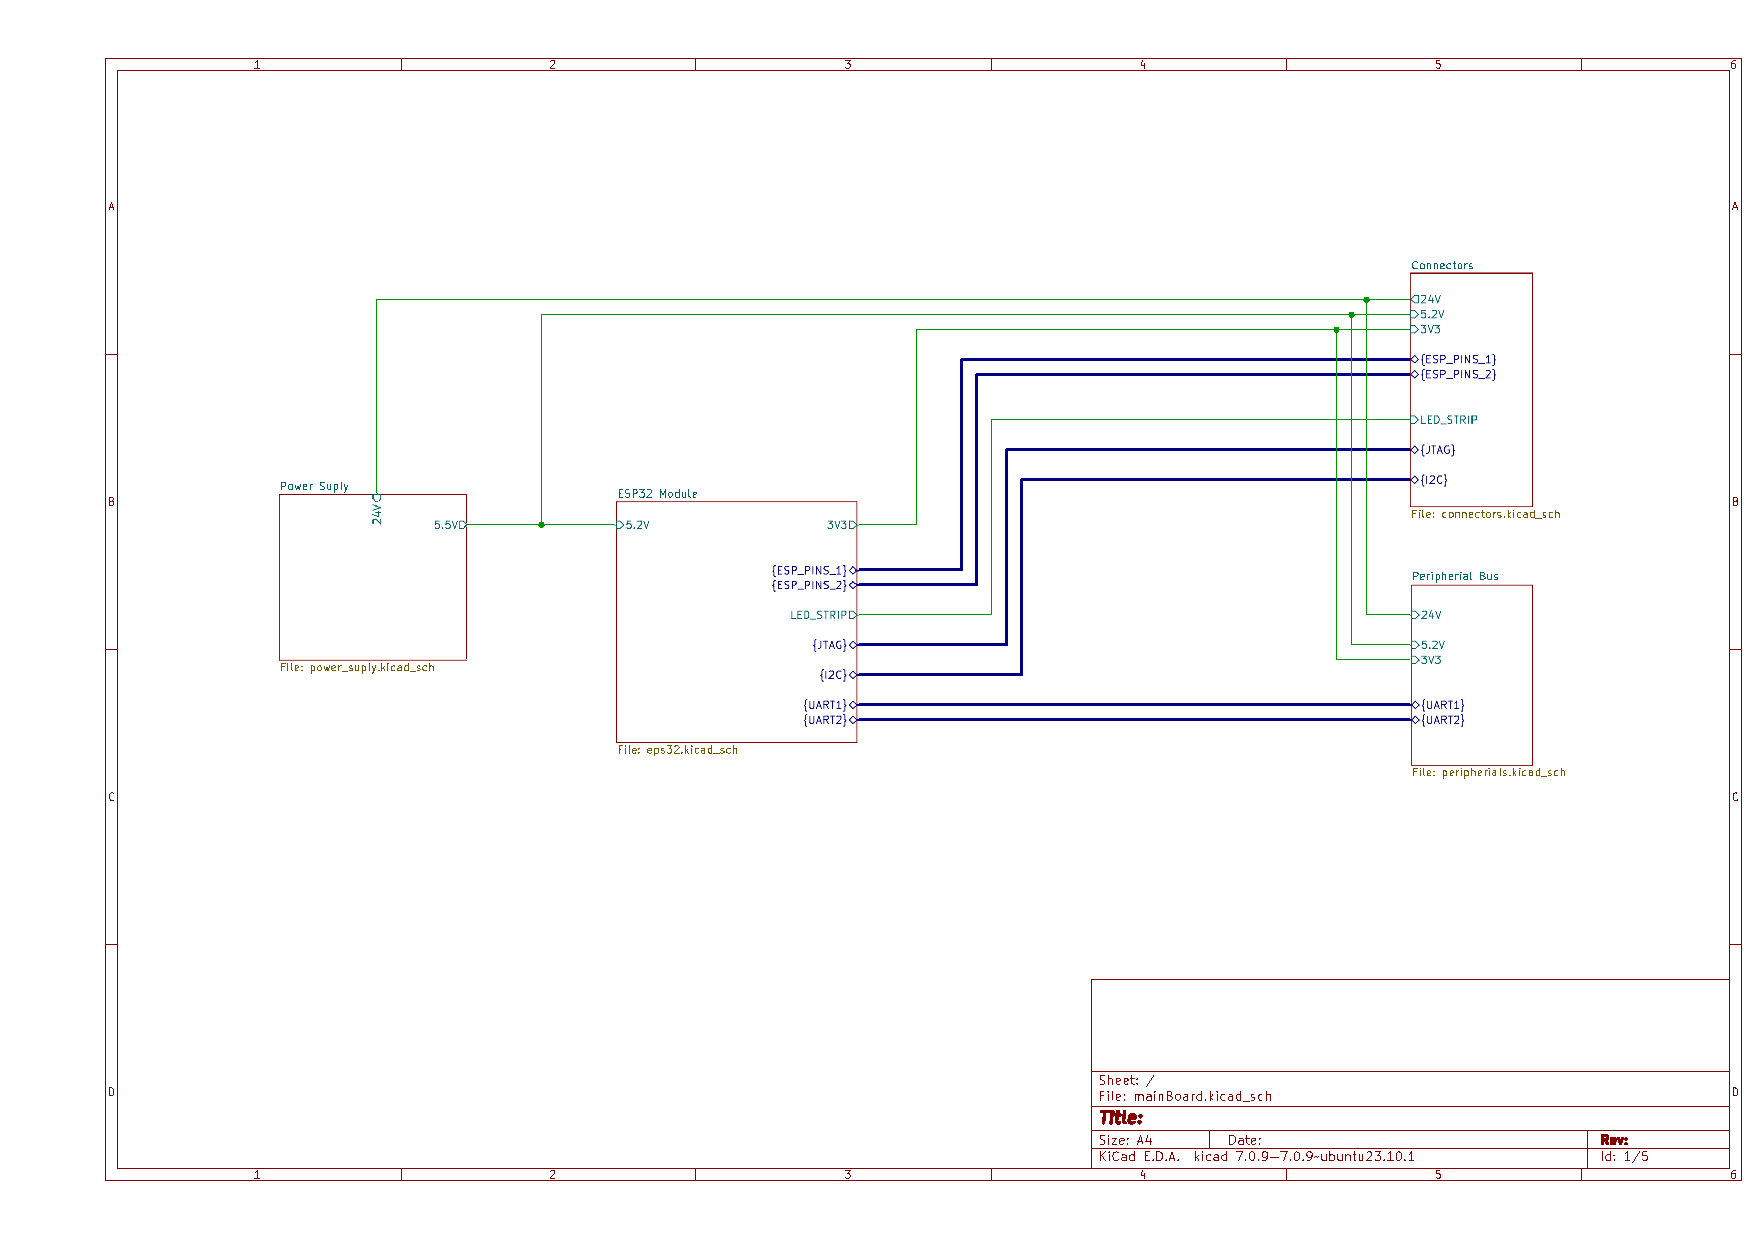
\includegraphics
	[
		width=\textheight, height=0.9\textwidth, keepaspectratio,
		page=1, 
		angle=90,
		trim=1.5cm 1cm 0cm 1cm, 
		clip
	]{obrazky/exportovane/main-board-schematic.pdf}

	\section{Zapojení MCU}
\label{priloha:schema-ridici-jednotka-mcu}
	% trim=left bottom right top
	\includegraphics
	[
		width=\textheight, height=\textwidth, keepaspectratio,
		page=2, 
		angle=90,
		trim=1.5cm 1cm 0cm 1cm, 
		clip
	]{obrazky/exportovane/main-board-schematic.pdf}

	\section{Napájecí obvod}
\label{priloha:schema-ridici-jednotka-napajeci-obvod}
	% trim=left bottom right top
	\includegraphics
	[
		width=\textheight, height=\textwidth, keepaspectratio,
		page=3, 
		angle=90,
		trim=1.5cm 1cm 0cm 1cm, 
		clip
	]{obrazky/exportovane/main-board-schematic.pdf}

	\section{Konektory}
\label{priloha:schema-ridici-jednotka-konektory}
	% trim=left bottom right top
	\includegraphics
	[
		width=\textheight, height=\textwidth, keepaspectratio,
		page=4, 
		angle=90,
		trim=1.5cm 1cm 0cm 1cm, 
		clip
	]{obrazky/exportovane/main-board-schematic.pdf}

	\section{Sběrnice periferií}
	\label{priloha:schema-ridici-jednotka-periferie}
		% trim=left bottom right top
		\includegraphics
		[
			width=\textheight, height=\textwidth, keepaspectratio,
			page=5, 
			angle=90,
			trim=1.5cm 1cm 0cm 1cm, 
			clip
		]{obrazky/exportovane/main-board-schematic.pdf}


\chapter{Schéma modulu periferií}
\label{priloha:schema-modul-periferii}
	% trim=left bottom right top
	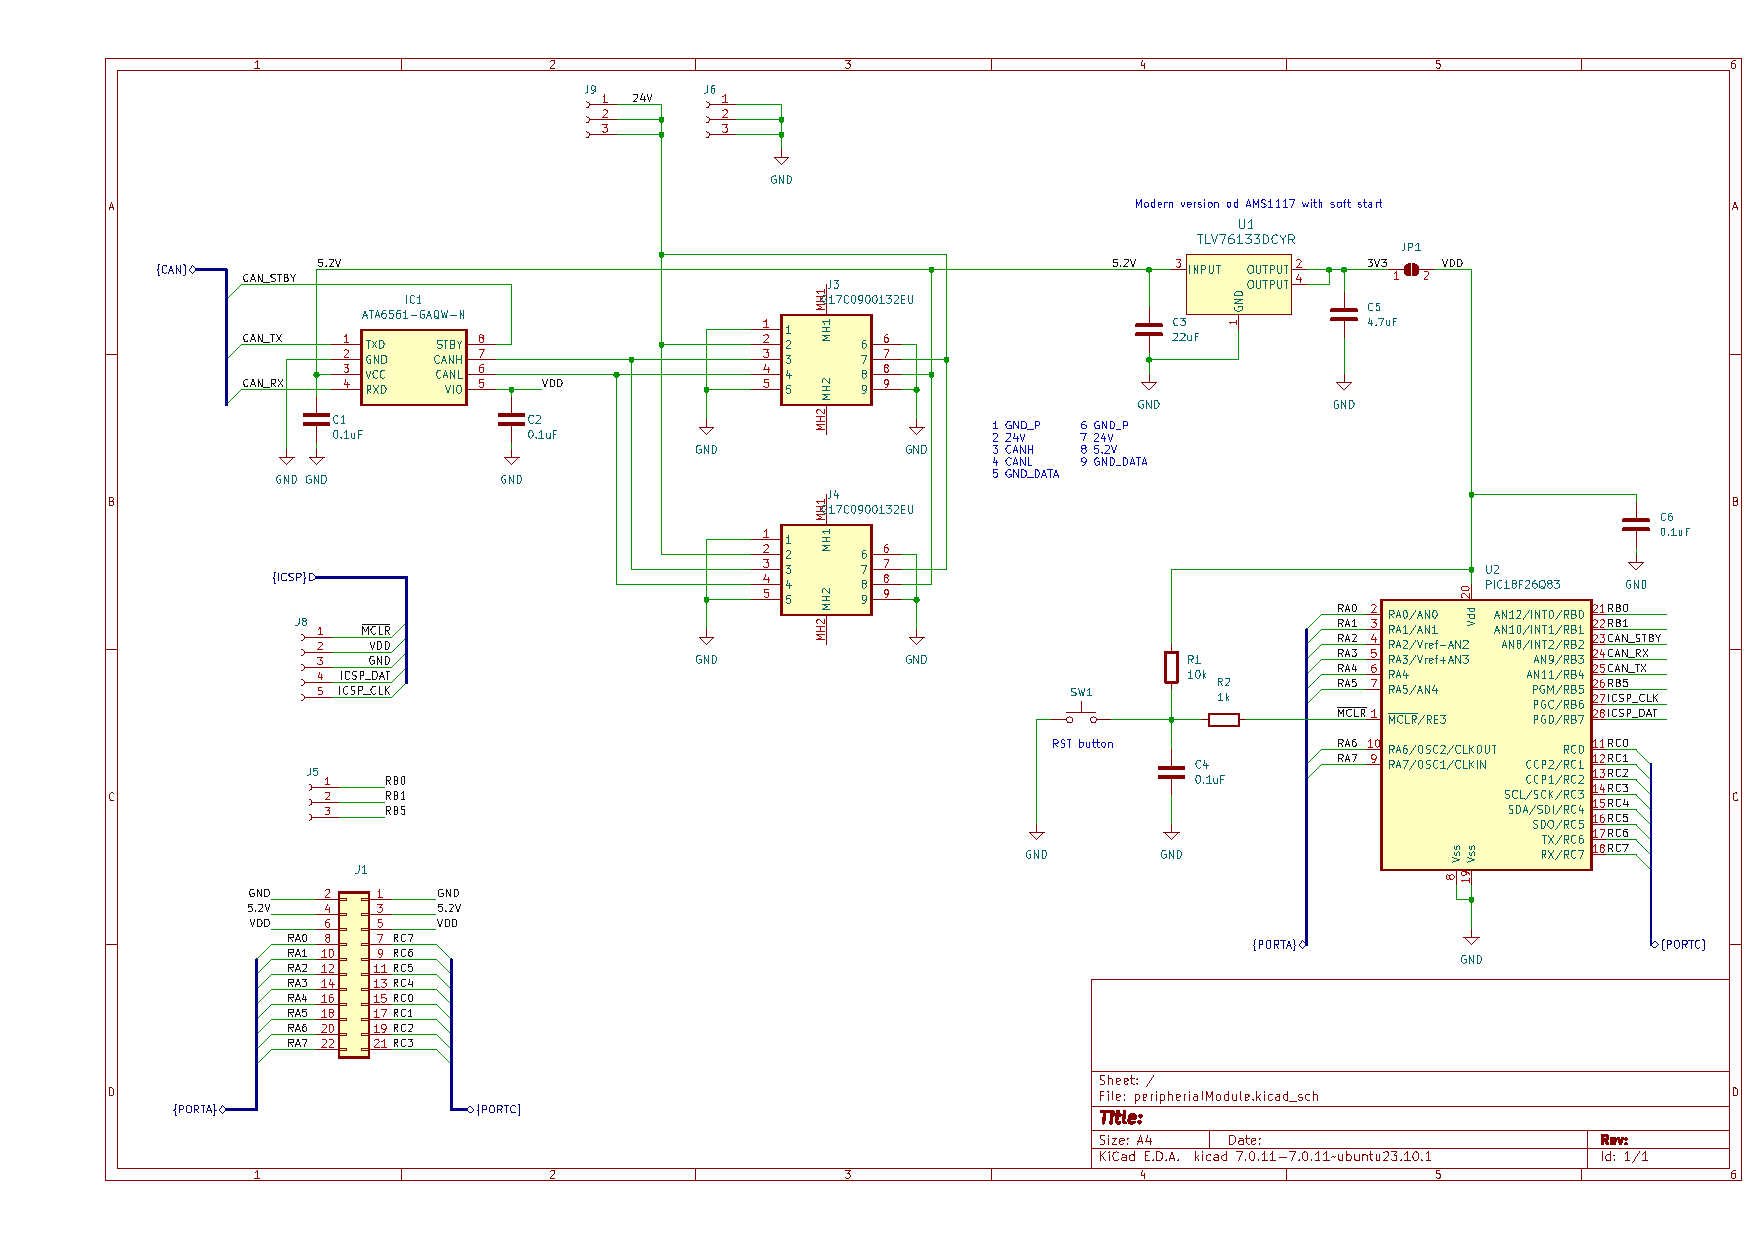
\includegraphics
	[
		width=\textheight, height=\textwidth, keepaspectratio,
		page=1, 
		angle=90,
		trim=1.5cm 1cm 0cm 1cm, 
		clip
	]{obrazky/exportovane/peripherial-module-schematic.pdf}

\chapter{Schéma modulu LED osvětlení}
\label{priloha:schema-led-board}
	% trim=left bottom right top
	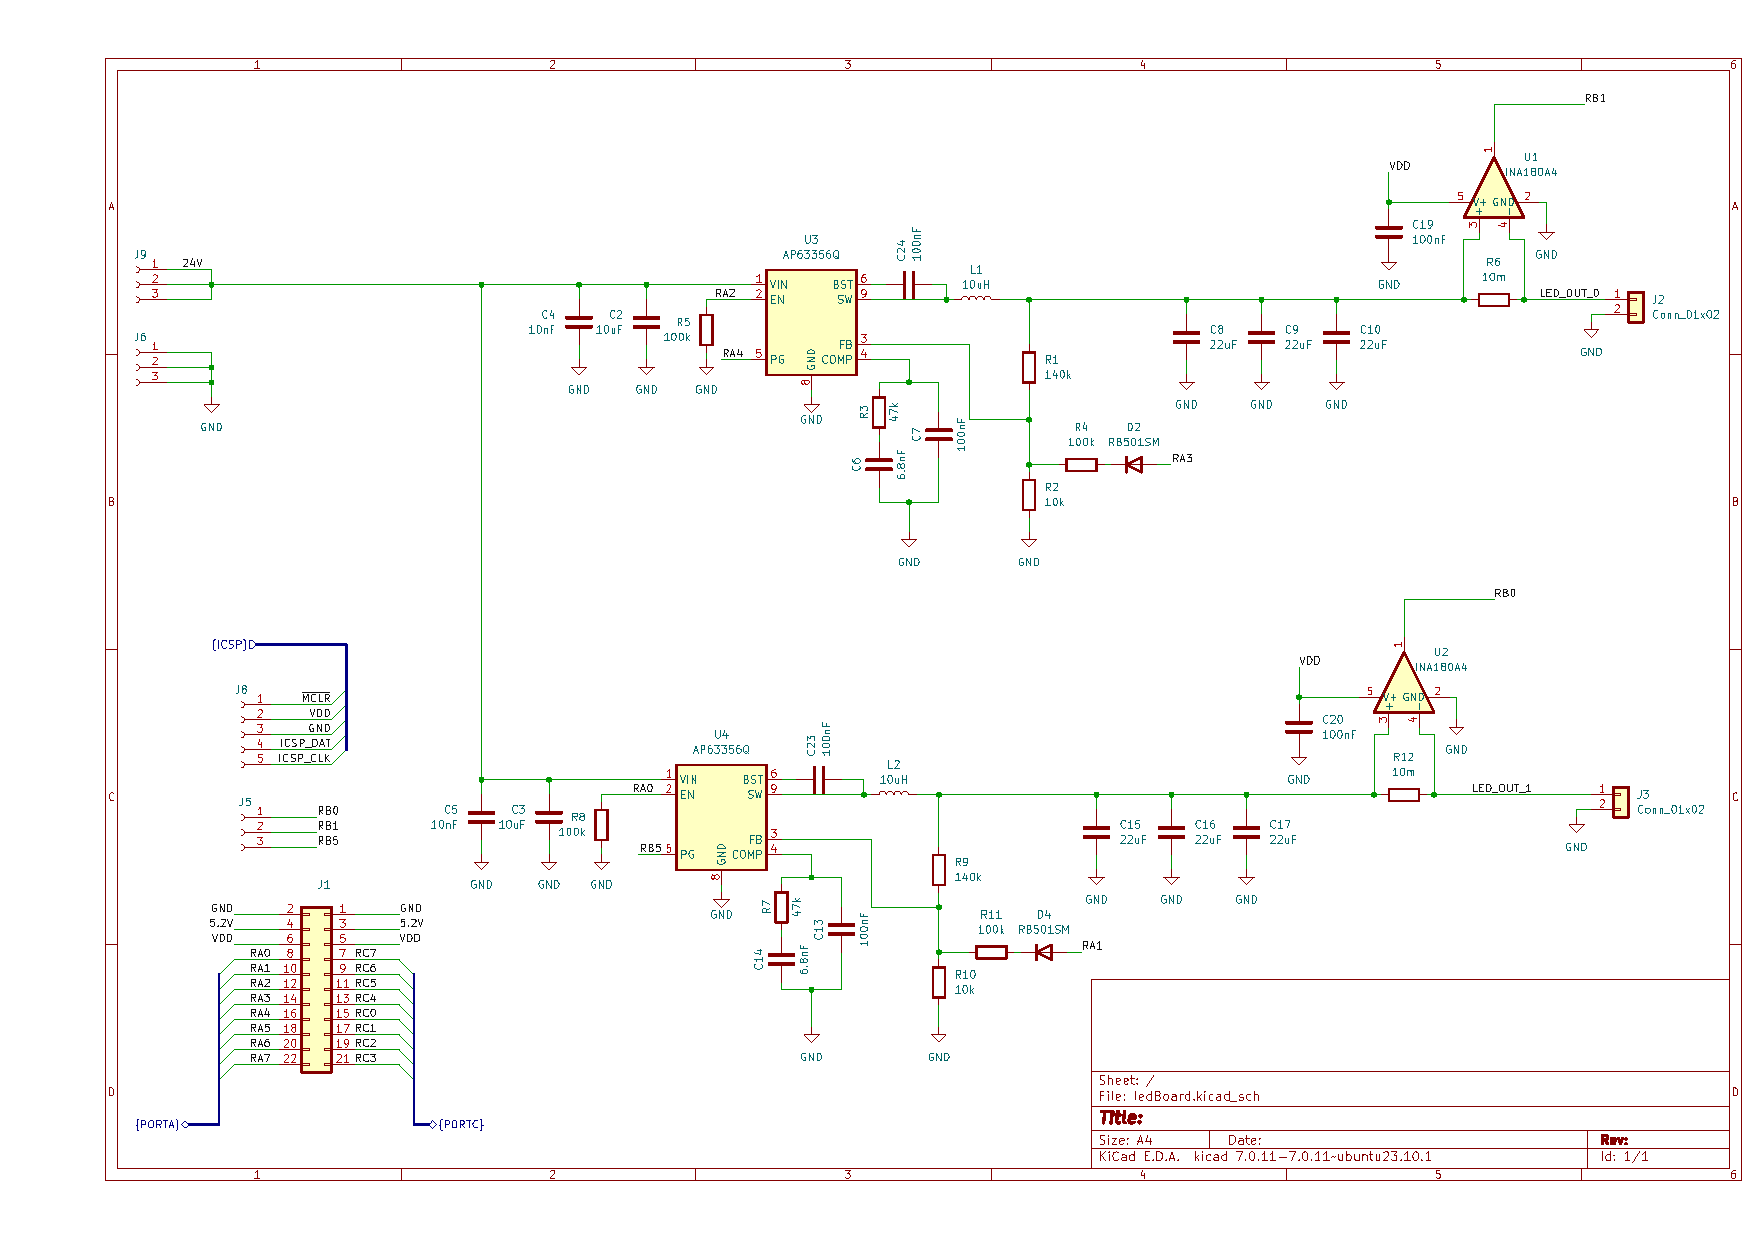
\includegraphics
	[
		width=\textheight, height=\textwidth, keepaspectratio,
		page=1, 
		angle=90,
		trim=1.5cm 1cm 0cm 1cm, 
		clip
	]{obrazky/exportovane/led-board-schematic.pdf}

\end{document}